\documentclass[handout, 10pt]{beamer}

%\usepackage[backend=bibtex,firstinits=true,style=verbose-inote,citestyle=authortitle]{biblatex}
\usepackage{bm}
\usepackage{graphicx}
\usepackage{subcaption}
\usepackage{amsmath}
\usepackage{amsfonts}
\usepackage{makecell}
\usepackage{filecontents}
\usepackage{biblatex}
\usepackage{xcolor}
% \newcommand{\expect}[2][]{
\ifthenelse{\equal{#1}{}}{
\mathbb{E}\left[#2\right]
}{
\underset{#1}{\mathbb{E}}\left[#2\right]
}}

\newcommand{\cov}[2][]{
\ifthenelse{\equal{#1}{}}{
\text{Cov}\left[#2\right]
}{
\underset{#1}{\text{Cov}}\left[#2\right]
}}


\newcommand{\var}[2][]{
\ifthenelse{\equal{#1}{}}{
\text{Var}[#2]
}{
\underset{#1}{\text{Var}}[#2]
}}

\newcommand{\loss}[2][]{
\ifthenelse{\equal{#1}{}}{
\mathcal{L}(#2)
}{
\mathcal{L}_{#1}(#2)
}}

\newcommand{\kl}[2]{
\text{D}_\text{KL}[#1 \parallel #2]
}

\newcommand{\R}{\mathbb{R}}
%\newcommand{\Prob}{\mathbb{P}}

\newcommand{\1}[1]{\mathds{1}\{#1\}}


%\usecolortheme{dolphin}
\setbeamertemplate{navigation symbols}{}
\setbeamertemplate{section in toc}{\inserttocsectionnumber.~\inserttocsection}

\begin{filecontents*}{references.bib}
@inproceedings{
OrderedNeurons,
title={Ordered Neurons: Integrating Tree Structures into Recurrent Neural Networks},
author={Yikang Shen and Shawn Tan and Alessandro Sordoni and Aaron Courville},
booktitle={International Conference on Learning Representations},
year={2019},
url={https://openreview.net/forum?id=B1l6qiR5F7},
}
\end{filecontents*}

\addbibresource{references.bib}


\title{Ordered Neurons: Integrating Tree Structures into Recurrent Neural Networks\footnote{\citepaper{OrderedNeurons}}}
%\subtitle{}
%\author{Ivan Skorokhodov}
%\date{}
%\logo{
\includegraphics[height=1cm]{images/ipavlov-logo.png}}

\newcommand{\citepaper}[1]{\citetitle{#1} by \citeauthor{#1}}

%\graphicspath{{./images}}

%\usetheme{lucid}
\begin{document}

\begin{frame}
    \titlepage
\end{frame}

\begin{frame}{Overview}
    \begin{itemize}
        \item\pause Human language has a tree-like structure
        \begin{figure}
            \centering
            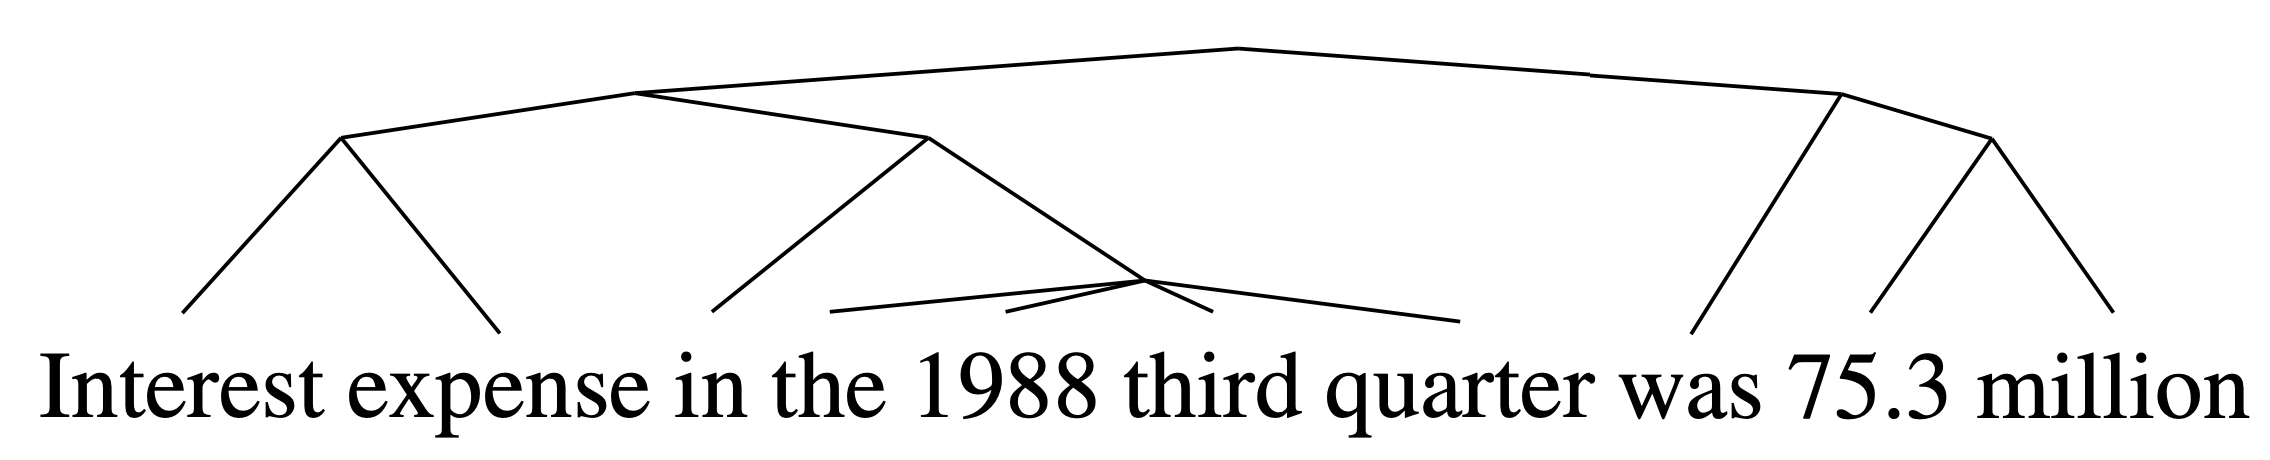
\includegraphics[width=0.5\textwidth]{images/tree-structure.png}
        \end{figure}
        \item\pause Human brain can infer it without any parse trees supervision
        \item\pause How can we force neural networks to acquire this structure without supervision as well?
        \item\pause Authors propose a specific inductive bias to do that:
        \begin{itemize}
            \item\pause divide a hidden state in a LSTM cell into chunks, each chunk keeps a hidden state for its own tree level
            \item\pause implement such a mechanism that can erase higher-level nodes only when all lower-level nodes are erased
            \item\pause this mechanism works by making forget/inputs gates of higher level nodes be dependent on the corresponding gates of lower-level ones
        \end{itemize}
        \item\pause They obtained good results for several tasks
    \end{itemize}
\end{frame}

\begin{frame}{Vanilla LSTM}
\pause
LSTM cell at timestep $t$ takes an input $x_t$, updates its cell state $c_t$ and hidden state $h_t$ in the following way:
\begin{enumerate}
    \item\pause Compute the following quantities:
    \begin{enumerate}
        \item\pause $f_{t}=\sigma\left(W_{f} x_{t}+U_{f} h_{t-1}+b_{f}\right)$ --- ``forget gate'' to erase $c_{t-1}$;
        \item\pause $i_{t}=\sigma\left(W_{i} x_{t}+U_{i} h_{t-1}+b_{i}\right)$ --- ``input gate'' to erase new \textit{raw} cell state $\hat{c}_t$
        \item\pause $o_{t}=\sigma\left(W_{o} x_{t}+U_{o} h_{t-1}+b_{o}\right)$ --- ``output gate'' to erase new hidden state $h_t$
    \end{enumerate}
    \item\pause Then compute the following quantities
    \begin{enumerate}
        \item\pause $\hat{c}_{t}=\tanh \left(W_{c} x_{t}+U_{c} h_{t-1}+b_{c}\right)$ --- new ``raw'' cell state
        \item\pause $c_t = f_t \circ c_{t-1} + i_t \circ \hat c_t$ --- new cell state
        \item\pause $h_{t}=o_{t} \circ \tanh \left(c_{t}\right)$ --- new hidden state
    \end{enumerate}
\end{enumerate}

\pause
Authors change the gating mechanism in such a way that erasement now occurs under some hierarchy.
\end{frame}


\begin{frame}{ON-LSTM (1/3)}
\begin{itemize}
    \item\pause Imagine that we have some arbitrary tree and we observe only leaves (i.e. our model takes leaves as inputs one by one)
    \item\pause At each timestep, we want to keep information not only about a leaf node, but also about every node on the path up to the root
    \item\pause Let's store the information about each node of a path in a separate chunk of our state vector:
    \begin{equation*}
        \bm v = [
        \underbrace{v_1^{(0)}, v_2^{(0)}, ..., v_m^{(0)}}_\text{leaf state},
        \underbrace{v_1^{(1)}, v_2^{(1)}, ..., v_m^{(1)}}_\text{leaf's parent state},
        ...,
        \underbrace{v_1^{(L)}, v_2^{(L)}, ..., v_m^{(L)}}_\text{root state},
        ]
    \end{equation*}
    \item\pause We know that erasing is the core operation in LSTM to update its state
    \item\pause So now we want a mechanism that would erase a higher level state only if all lower-level states are erased as well
\end{itemize}
\end{frame}


\begin{frame}{ON-LSTM (2/3)}
\begin{itemize}
\item\pause To implement the desired mechanism, our erasement vector $\bm g$ for $\bm v$ should have the following structure:
\[
g = [0, 0, 0, 0, ...., 1, 1, 1],
\]
i.e. we have a segment of zeros followed by a segment of ones.
\item\pause The idea is based on a novel activation function \textcolor{blue}{cumax}:
\begin{equation*}
    \text{cumax}(...) = \text{cumsum}(\text{softmax}(...))
\end{equation*}
(it operates on vectors instead of scalars).
\item\pause Let $d$ be a \textit{split point}, i.e. a number when the first ``1'' occured.
\item\pause Then $d$ follows categorical distribution and we can model it with softmax:
\[
p(d) = \text{softmax}(\hat{\bm d})
\]
\end{itemize}
\end{frame}

\begin{frame}{ON-LSTM (3/4)}
\begin{itemize}
    \item\pause Using $d$ we can compute $p(g_k = 1)$, i.e. a probability of $k$-th element of $g$ being equal to 1:
\[
p(g_k = 1) = p(d \leq k) = \sum_{i \leq k} p(d = i)
\]
    \item\pause To compute a vector of probabilities $[p(g_1 = 1), ..., p(g_n = 1)]$ we need to apply cumax on $\hat{\bm d}$:
\[
p(\bm g) = \text{cumax}(\hat{\bm d})
\]
    \item\pause So we use a continuous relaxation for erasement operation (like in a vanilla LSTM) and erase a part of $\bm v$ by computing
    \[
        p(\bm g) \circ \bm v
    \]
    \item\pause In this way, higher level segments are erased only if all the lower-level ones are erased
\end{itemize}
\end{frame}


\begin{frame}{ON-LSTM (4/5)}
\pause
Imagine that at the current timestep we are at some level $\ell$, i.e.:
    \begin{itemize}
        \item we are going to ``close'' the branch of height $\ell$
        \item we are going to erase the state below it
        \item we are going to keep all the higher-level context
    \end{itemize}
\end{frame}

\begin{frame}{ON-LSTM (5/6)}
\pause First we should compute the master gates:
    \begin{enumerate}
        \item\pause $\tilde{f}_{t}=\operatorname{cumax}\left(W_{\tilde{f}} x_{t}+U_{\tilde{f}} h_{t-1}+b_{\tilde{f}}\right)$ --- a mask, which discards all lower-level elements
        \item\pause $\tilde{i}_{t}=1-\operatorname{cumax}\left(W_{\tilde{i}} x_{t}+U_{\tilde{i}} h_{t-1}+b_{\tilde{i}}\right)$ --- a mask which keeps only lower-level elements
        \item\pause Compute the mask for the current-level segment $\omega_{t} =\tilde{f}_{t} \circ \tilde{i}_{t}$.
    \end{enumerate}

These vectors would look like this (ideally):
\begin{equation}
\begin{aligned}
%\tilde{f}_{t} &= [
%        \underbrace{0, 0, 0}_\text{leaf mask},
%        \underbrace{0, 0, 0}_\text{leaf's parent mask},
%        \underbrace{1, 1, 1}_\text{current level $\ell$ mask},
%        \underbrace{1, 1, 1}_\text{root mask},
%        ] \\
%\tilde{i}_{t} &= [
%        \underbrace{1, 1, 1}_\text{leaf mask},
%        \underbrace{1, 1, 1}_\text{leaf's parent mask},
%        \underbrace{1, 1, 1}_\text{current level $\ell$ mask},
%        \underbrace{0, 0, 0}_\text{root mask},
%        ] \\
%\omega_{t} &= [
%        \underbrace{0, 0, 0}_\text{leaf mask},
%        \underbrace{0, 0, 0}_\text{leaf's parent mask},
%        \underbrace{1, 1, 1}_\text{current level $\ell$ mask},
%        \underbrace{0, 0, 0}_\text{root mask},
%        ]
\tilde{f}_{t} &= [0, 0, 0, 0, 0, \textcolor{blue}{1}, \textcolor{blue}{1}, 1, 1] \\
\tilde{i}_{t} &= [1, 1, 1, 1, 1, \textcolor{blue}{1}, \textcolor{blue}{1}, 0, 0] \\
\omega_{t} &=    [0, 0, 0, 0, 0, \textcolor{blue}{1}, \textcolor{blue}{1}, 0, 0]
\end{aligned}
\end{equation}


%\begin{equation}
%\begin{aligned}
%\omega_{t} &=\tilde{f}_{t} \circ \tilde{i}_{t} \\
%\hat{f}_{t} &=f_{t} \circ \omega_{t}+\left(\tilde{f}_{t}-\omega_{t}\right)=\tilde{f}_{t} \circ\left(f_{t} \circ \tilde{i}_{t}+1-\tilde{i}_{t}\right) \\
%\hat{i}_{t} &=i_{t} \circ \omega_{t}+\left(\tilde{i}_{t}-\omega_{t}\right)=\tilde{i}_{t} \circ\left(i_{t} \circ \tilde{f}_{t}+1-\tilde{f}_{t}\right) \\
%c_{t} &=\hat{f}_{t} \circ c_{t-1}+\hat{i}_{t} \circ \hat{c}_{t}
%\end{aligned}
%\end{equation}
\end{frame}


\begin{frame}{ON-LSTM (6/6)}
Then we update the states the following way:
\begin{enumerate}
    \setcounter{enumi}{2}
    \item\pause Compute old element-wise forget and inputs gates $f_t, i_t$ and new raw cell state $\hat{c}_t$ without changes.
    \item\pause $\hat{f}_{t} =f_{t} \circ \omega_{t}+(\tilde{f}_{t}-\omega_{t})$ --- forget gate that affects current level $\ell$, erases all lower-level elements and keeps all higher-level elements
    \item\pause $\hat{i}_{t} =i_{t} \circ \omega_{t}+(\tilde{i}_{t}-\omega_{t})$ --- forget gate that affects current level $\ell$, erases all higher-level elements and keeps all lower-level elements
    \item\pause $c_{t} =\hat{f}_{t} \circ c_{t-1}+\hat{i}_{t} \circ \hat{c}_{t}$ --- new cell state
    \item\pause $h_t$ is computed without changes
\end{enumerate}

In this way we have updated only those part of the hidden state which corresponds to some specific level of a tree.
\end{frame}


\begin{frame}{Conclusion}
    \begin{itemize}
        \item LSTM still performs better for short-term dependencies
        \item We repeat each dimension C times, before the element-wise multiplication    
        \item It is interesting to see that there is room for exploration even in such an extensively explored model as LSTM
        \item Can we bring the idea into Transformers? Graph NNs?
    \end{itemize}
\end{frame}
\end{document}
